\chapter{Implementation}

\mytodo{Introduce the project, say it is written in C, point to the github repo url, etc...}

\section{Introduction to CPLEX}

\mytodo{Explain what is CPLEX, academic license, url where it can be downloaded etc}


\section{Full static model}

\begin{align}
	\min_{x,y} \quad z(x, y) & =  \sum_{i \in V} \sum_{\substack{j \in V                                                                                                   \\ j \ge i + 1}} d_{ij} x_{ij} - \sum_{i \in V} p_i y_i \label{eq:obj-function}\\
	                         & y_0 = 1                                           & \label{eq:full-static-model-depot-part-of-tour-constraint}                              \\
	                         & \sum_{j \in \delta(i)}       x_{ij}    = 2        & \quad \forall i \in V         \label{eq:full-static-model-flow-conservation-constraint} \\
	                         & B \le   \sum_{i \in V} q_i y_i   \le Q            & \label{eq:full-static-model-resource-upper-bound-constraint}                            \\
	                         & x_{ij}                   \in \lbrace 0, 1 \rbrace & \quad \forall (i, j) \in E               \label{eq:full-static-model-x-mip-var-bounds}  \\
	                         & y_{i}                    \in \lbrace 0, 1 \rbrace & \quad \forall i \in V,\ i \ge 1          \label{eq:full-static-model-y-mip-var-bounds}
\end{align}

which follows closely the full IP formulation presented in \eqref{eq:obj-function} without the GSECs.
We also added a non strictly necessary lower bound on the served demand, which details were already discussed earlier in Section \ref{sec:demand-lower-bound}.

\section{Cutoff values}


\subsection{Upper cutoff value}
Since we're interested in solving the CPTP in the context of pricing for the CVRP, we're interested only in valid tours achieving a strictly negative objective value.
Therefore we can specify an upper cutoff for objective function $z(x, y)$:

\begin{equation}
	z(x, y) \le 0 - \epsilon_{\mt{ct}}
\end{equation}

where $\epsilon_{\mt{ct}} \in \R$ is the upper cutoff tolerance, in our implementation we picked $\epsilon_{\mt{ct}} = 10^{-6}$, which is the default used in BapCod.

The upper cutoff value can improve the linear relaxation and reduce the number of branch and bound nodes that need to be explored, especially when the MIP solver cannot infer any good starting primal solution.

\subsection{Lower cutoff value}
A good lower cutoff value on the objective function can improve the linear relaxation, and reduce the number of branch and bounds nodes that need to be explored.
When combined with an upper cutoff value, and a good set of warm start solutions it can help to start the solution process with an already relatively closed gap.

A lower cutoff value can be obtained by any feasible dual solution.
For example we could use the method briefly described in Section \ref{sec:cptp-simple-dual-formulation} to obtain a good feasible dual solution.
At the time of writing of this draft report (late Jan, firsts Feb 2022) the method described in Section \ref{sec:cptp-simple-dual-formulation} was not extensively explored.

Instead we opted for a much simpler dual bound:

\begin{equation}
	z(x, y) \ge - \sum_{i \in V} p_i
\end{equation}

which is a trivial and weak bound, and in pretty much all cases, is easily beaten by a better alternative computed from the preprocessing stage of a standard MIP solver.

\section{Warm start}

Heuristic algorithms can be used to provide good feasible starting primal solutions to the MIP.
A CPTP problem has many similarities with TSP, therefore heuristics for the TSP, if slightly adapted, ca be applied successfully to this problem domain.
Much work was dedicated in studying good heuristics for the TSP, see \cite{rosenkrantz_analysis_1977}, \cite{johnson_traveling_1997}, \cite{laporte_traveling_1992}, \cite{johnson_experimental_2007}, \cite{hoffman_traveling_2013}.

In the remainder of this section we explain the implemented warm start procedure which is characterized by two stage: a constructive insertion heuristic stage followed by a 2-OPT refinement stage.

\subsection{Insertion heuristic}
\cite{rosenkrantz_analysis_1977} do a fantastic job describing the insertion heuristic algorithm for the TSP and various facets in which it can be implemented.
The insertion heuristic algorithm can construct a new feasible primal solutions in $\Theta(N^2)$ time.

In this section, we will focus on adapting the insertion heuristic for the TSP so that it can be applied to CPTP problems.
Start by selecting two distinct nodes $s, t \in V,\ q_s + q_t \le Q$ and use these two nodes to form a tour back-to-back.

The insertion heuristic algorithm works iteratively where at each step of the iteration we always have a valid tour, which is not necessarily feasible for the CPTP.
At the end of the whole algorithm, we will obtain a valid tour which is also feasible for the CPTP.
Let's define $Q_t$ as the total demand served in the current tour.
At each iteration, choose a vertex $a$ that belongs to the current tour and a vertex $h$ which is not yet part of the tour.
Let's define $a_s$ as the successor of node $a$ in the current tour.
The idea is to try to insert $h$ in the current tour, by deleting edge $(a, a_s)$, and inserting edges $(a, h),\ (h, a_s)$ but only if $h$ must be inserted or improves over the current tour.
Let's define the extra mileage as
:
\begin{equation}
	\Delta_m(h, a) =
	\begin{cases}
		d_{ah} + d_{ha_s} - d_{aa_s} - p_h, & \texttt{if } Q_t + q_h \le Q \\
		\infty,                             & \texttt{otherwise}
	\end{cases}
\end{equation}

which represents the delta cost in inserting $h$ as the successor of $a$.
A node $h$ is a good candidate for insertion if at least one of the following conditions is true:
\begin{enumerate}
	\item $\Delta_m(h, a) < 0$, i.e. inserting $h$ improves over the current tour.
	\item $h = 0$, i.e. $h$ is the depot node. The depot node at some point must be inserted regardless whether it is improving or not.
	      Note that by convention we have defined $q_0 = 0$, therefore $Q_t + q_0 \le Q$ is always satisfied for the depot node.
	\item The number of visited nodes in the current tour is $2$ and $Q_t + q_h \le Q$.
\end{enumerate}

In our implementation we employed a cheapest insertion scheme, therefore the pair $(h, a)$ for the current insertion iteration is picked such that it minimizes as much as possible the extra mileage $\Delta_m(h, a)$.
The iteration stops when no more valid $h$ vertices can be found for insertion.
It may happen that no valid $h$ can be found, yet the current tour length is $2$.
In this very unlikely scenario, we can conclude that the CPTP formulation does not admit any feasible solution before even solving the IP formulation.

In our implementation we picked $s = 0$ and $t \in V_0$, such that $q_s + q_t \le Q$.
This allows us to generate $O(N)$ good feasible primal solutions using insertion heuristic in $O(N^3)$ time.

\subsection{2-OPT refinement}
In our implementation, each solution produced from the insertion heuristic is further improved using a 2-OPT refinement procedure.
The 2-OPT algorithm is a heuristic local-search hill-climbing procedure proposed originally for the TSP in \cite{flood_traveling-salesman_1956}, \cite{croes_method_1958}.

An application of the 2-OPT algorithm works iteratively requiring $\Omega(N^2)$ time.
Unfortunately, as it is pointed out in \cite{chandra_new_1999}, the 2-OPT algorithm may in the worst case take an exponential number of iterations when fed with purposely artificially constructed instances.
Although this is bad news, it is also worth pointing out that this rarely occur in practice, as the probabilistic average number of iterations required for 2-OPT is at most polynomial.

Each iteration of the 2-OPT procedure searches for an existing edge crossing, and if any exists, it performs a 2-OPT exchange to undo it.
A 2-OPT exchange always maintain the original feasibility, therefore if the 2-OPT algorithm is applied on a feasible solution, it will remain feasible at the end of the whole procedure.
We briefly describe the 2-OPT exchange.
Let $a, b \in V$ be two vertices visited in the current tour, and let's use $a_s, b_s \in V$ to denote respectively the successor of $a$ and $b$ in the current tour.
A 2-OPT exchange removes edges $(a, a_s)$, $(b, b_s)$ in favor of $(a, b)$, $(a_s, b_s)$ but only if the delta distance defined as:

\begin{equation}
	\Delta(a, b) = d_{ab} + d_{a_sb_s} - d_{aa_s} - d_{bb_s}
\end{equation}

satisfies $\Delta(a, b) < 0$.
If this is the case, performing a 2-OPT exchange over vertices $(a, b)$ can improve the current tour.
After the 2-OPT exchange it is necessary to reverse part of the tour characterized from the head $a_s$ and tail $b$: $[a_s, \dots, b]$.

In our implementation we scan for vertices $a, b$ achieving the cheapest exchange, i.e. for which $\Delta(a, b)$ is minimized across all possible valid choices of $a, b$.


\section{Separation techniques}

Inequality separation is a problem which consists in finding strong valid violated inequalities so that such inequalities can be embedded inside a Branch\&Cut framework.
Integral inequality separation is concerned in determining violated inequalities for the original IP model.
Integral inequalities separation is usually much easier to perform, and can be seen as a procedure to dynamically generate necessary constraints that would otherwise be impossible to insert statically in a MIP model.
Fractional inequality separation, instead is usually harder to perform, and it is concerned in finding strong violated inequalities for fractional solution stemming out from a linear relaxation of a MIP formulation.

In this thesis we are treating a CPTP problem, and more precisely, we are concerned in separating the GSEC, GLM, RCI inequalities presented in Sections \ref{sec:gsec-inequality}, \ref{sec:additional-valid-inequalities}.
This is achieved by finding a set $S \subseteq V_0$, through the usage of appropriate algorithms, that violates any valid inequality.

All the cuts that we implemented, are backed by the same shared separation procedure for both integral solutions and for fractional solutions.
In the next two sections, we describe the common separation procedure used to find good $S \subseteq V_0$ sets.
Then for each cut, we describe how $S$ is used for generating the inequality and when each cut is reported to the MIP solver and when it is instead ignored.

\subsection{Integral separation}
The integral separation procedure is the most important, as this procedure is necessary to generate GSEC cuts dynamically, and to avoid that the MIP solver produces solutions with spurious subtours.
Assume that the MIP solver finds an optimal integer solution $x^* \in \{0, 1\}, y^* \in \{0, 1\}$ that violates a GSEC constraint.
If $x^*$ violates at least a GSEC, it is easy to see that the solution models at least a spurious unconnected subtour that needs to be removed.
In order to detect unconnected subtours, we need first to determine the connected components induced from the $x^*$ solution.

Let $C = \{-1, 0, \dots, n_c - 1\}$ be the connected components formed with $n_c \ge 1$.
By definition, we use the sentinel value $-1$ to denote that a node $i$ does belong to a singleton connected component containing only $i$ itself.
We are only interested in modeling major connected components, i.e. containing at least two vertices, thus we ignore singleton connected components.
Thus, the $n_c$ represents the number of major connected components, i.e. the number of subtours formed in the current integral solution.
Let $cc(i) \in C$ be an array which for each vertex $i \in V$ it encodes to which connected component it belongs to.
Note that the depot node always belongs to a connected component, therefore by definition we fix $cc(0) = 0$, and $c(i) = -1  \quad \forall i \in V_0 \mid y_i = 0$.
The connected components can be computed by a simple depth first search traversal, for which a pseudocode is provided in Algorithm \ref{src:cc-dfs}.

\begin{algorithm}
	\caption{An algorithm for computing the connected components through a DFS traversal}
	\label{src:cc-dfs}
	\KwData{$x^*, y^* \in \{0, 1\}$: current optimal integer solution}
	\KwResult{$n_c$: number of subtours formed}
	\KwResult{$cc[i] \in C$: connected component of $\forall i \in V$}
	$cc[i] \gets -1 \quad \forall i \in V$\;
	$nc \gets 0$\;
	\For{$i\gets0$ \KwTo $N$}{
		\If{$cc[i] < 0, y_i \ge 0.5$}{
			\Comment{Found a non visited subtour}
			$cc[i] \gets n_c$\;
			$u \gets -1$\;
			\Comment{Traverse the subtour}
			\Do{$u \ge 0$}{
				$v \gets -1$\;
				\For{$j \in V \mid (u, j) \in E, cc[j] < 0, x^*_{uj} \ge 0.5$}{
					\Comment{The body of this loop will execute only once}
					$cc[j] = n_c$\;
					$v \gets j$\;
				}
				$u \gets v$
			}
			$n_c \gets n_c + 1$\;
		}
	}

	\Comment{Validate some invariants}
	\Assert{$n_c \ge 0$}\;
	\Assert{$c[0] = 0$}\;
	\Assert{$c[i] = -1 \quad \forall i \in V_0 \mid y_i < 0.5$}\;
	\Assert{$c[i] \ge 0 \quad \forall i \in V_0 \mid y_i \ge 0.5$}\;
	\Comment{Done: terminate}
	\Return{$n_c, cc$}
\end{algorithm}
Then any valid set $S \in V_0$ can be computed in the following way from a MIP integer solution:

\begin{equation}
	S \subseteq V_0 = \left\{ i \mid cc(i) = k  \right\}   \quad \forall k \in C, k \ge 0
\end{equation}

which implies that any major connected component that does not contain the depot node, can be used as a valid set $S \subseteq V_0$ for separating inequalities.
If $n_c = 1$ then no $S \subseteq V_0$ can be separated for this integral solution, which in our case simply means that the solution contains a single subtour, and does not violate any GSECs.


\subsection{Fractional separation}
Fractional separation is usually much harder and more computationally expensive to perform compared to integral separation.
A valid set $S \subseteq V$ can be separated by solving a max-flow problem between two arbitrary source and sink vertices $s, t$ on a fully connected directed graph.
Fractional separation is modeled through a directed symmetric flow network, where $x^*_{ij}$ constitutes the capacities of the flow network.

One important notice is that writing good max-flow algorithms that operate directly with floating point arithmetic can be difficult and error-prone, since discharging and removing flow from edges is not an exact procedure.
And it is possible to get stuck in long loops discharging atomically small quantity of flows.


A solution to the max-flow problem outputs a maxflow $f_{\mt{max}}(s, t)$ and a bipartition, also called "coloring", of the set $V$, namely two complementary sets $F_1(s, t), F_2(s, t)$ such that $F_1(s, t) \cup F_2(s, t) = V$ and $F_1 \cap F_2 = \emptyset$, and such that $s \in F_1(s, t),\ t \in F_2(s, t)$.
The $\delta(F_1(s, t))$ constitutes the min-cut induced from the solving the max-flow problem over $(s, t)$.
It is known that solving a maxflow problem guarantees the following two properties:

\begin{enumerate}
	\item Edges $\{ (i, j) \mid i \in F_1(s, t),\ j \in F_2(s, t) \}$ are saturated
	\item Edges $\{ (j, i) \mid i \in F_1(s, t),\ j \in F_2(s, t) \}$ are drained.
\end{enumerate}

therefore the following result holds:
\begin{align}
	\sum_{(i, j) \in \delta(F_1(s, t))} f_{ij} & = f_{\mt{max}}(s, t) \\
	\sum_{(i, j) \in \delta(F_2(s, t))} f_{ij} & = 0
\end{align}

where $f_{ij}$ denotes the flow along the edge $(i, j) \in V$ in the corresponding flow network.
Assuming we have already computed $F_1, F2$, a valid $S \subseteq V_0$ can then be picked such that:
\begin{equation}
	S \subseteq V_0 =
	\begin{cases}
		F_1(s, t), & \texttt{if } 0 \notin F_1 \\
		F_2(s, t), & \texttt{otherwise}
	\end{cases}
\end{equation}

This fractional separation framework based on max-flow computations, can separate up to $N^2 - N$ different $S \subseteq V_0$ sets, one for each possible choice of $s, t \in V, s \ne t$.
It is important to note that, since we are dealing with a symmetrical flow network, solving the maxflow problem between pairs $(s, t)$ and pair $(t, s)$ will output the same maxflow, i.e. $f_{\mt{max}}(s, t) = f_{\mt{max}}(t, s)$.
Although, and this is the more important aspect, the induced bipartitions in the general case are not guaranteed to be symmetric.
Namely, in the general case $F_1(s, t) \ne F_2(t, s)$ and $F_2(s, t) \ne F_1(t, s)$.
To see this is the case, this simple flow network:

\begin{figure}[H]
	\centering
	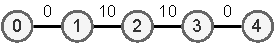
\includegraphics[width=6cm]{Imgs/single-path-flow-network.pdf}
\end{figure}

produces the same max flow when solving for $(0, 4)$ and $(4, 0)$ pair respectively, and produces $F_1(0, 4) = \{ 0\},\ F_2(0, 4) = \{ 1, 2, 3, 4\}$, $F_1(4, 0) = \{ 4 \},\ F_2(4, 0) = \{ 0, 1, 2, 3\}$, which clearly represent a non symmetric coloring.
This behaviour is a direct consequence that flow networks don't guarantee unique min-cuts.

In this thesis, we used the push relabel max flow algorithm first developed in \cite{goldberg_efficient_1997}, which is usually faster than more classical approaches such as the Ford-Fulkerson max-flow algorithm.
The push relabel max flow algorithm runs in $O(N^4)$ time, and when combined with an exhausitive enumeration over all possible choices of $s, t$, can take up to $O(N^6)$ time.

The Gomory-Hu tree, first presented in \cite{gomory_multi-terminal_1961}, provides a way to compute the all pairs $(s, t)$ max-flows using only $N$ main max-flow computations.
A Gomory-Hu tree can be seen as a data structure that represents a simpler reduced flow network, where max-flow computations become trivially solvable through a single iteration of the Ford-Fulkerson algorithm in $\Theta(N^2)$.
Combining Gomory-Hu trees and the push relabel max flow algorithm, an exhaustive enumeration of all possible $(s, t)$ vertices takes up to $O(N^5)$ time to build the tree, and further $\Theta(N^4)$ to query for all the possible $F_1(s, t), F_2(s, t)$ bipartitions.

In this implementation we employed the usage of both the push relabel algorithm, the Gomory-Hu tree and full enumeration of all possible $(s, t)$ vertices.
Since running this full enumeration over each fractional separation, turned out to be quite costly, we decided to amortize the cost over multiple iterations.
Namely, fractional separations iterations which are not multiple of $N$ become a no-op, no max-flow is performed, and therefore no set $S \subseteq V_0$ is separated.

While there may be other ways to separate sets $S \subseteq V_0$, the described approach works very well for the inequalities considered in this thesis.
This is very convenient because a single separation procedure for $S \subseteq V_0$ can be shared across all the inequalities, thus reducing computation time.
Other kinds of inequalities, which are not considered in this thesis, may benefit from other more elaborate separation techniques.

In the following sections we describe how we separate each inequality using the computed $S \subseteq V_0$.

\subsection{GSEC separation}

\subsubsection{GSEC integral separation}
This is the most important separation technique, since it is mandatory to solve the CPTP.


\subsection{GLM separation}

\subsection{RCI separation}
